%%%%%%%%%%%%%%%%%%%%%%%%%%%%%%%%%%%%%%%%%%%%%%%%%%%%%%%%%% 
\chapter{クイーン支配問題}\label{chap:background}
%%%%%%%%%%%%%%%%%%%%%%%%%%%%%%%%%%%%%%%%%%%%%%%%%%%%%%%%%% 

\section{支配集合問題}
無向グラフ$G=(V,E)$の頂点の部分集合$S\subset V$に対して,
任意の頂点$u \in V\setminus S$にも辺$(u,v) \in E$が存在し,
$v \in S$を満たすとき,
$S$を$G$の\textbf{支配集合 (dominating set)}という.
支配集合$S$の要素数を\textbf{サイズ}という.
 \begin{itemize}
  \item サイズが最小の支配集合を\textbf{最小支配集合}という.
  \item 最小支配集合のサイズをグラフ$G$の\textbf{支配数 (domination number)}という.
    本論文ではグラフ$G$の支配数を$\gamma(G)$で表す.
 \end{itemize}

グラフ$G$と正の整数$k$が与えられたとき,
サイズが$k$の$G$の支配集合が存在するかどうかを
判定する問題を\textbf{支配集合問題}という.
支配集合問題は\textbf{NP完全}に属する問題
であることが証明されている~\cite{Jhonson79}.
支配集合問題で,グラフの頂点を「町」,辺を「二つの町の間で電波の届く関係」とみなすと,
支配数の決定は電波塔の最適な配置に対応づけられる.
また,支配数や支配集合はスケジューリングなど多くの問題に応用されている
~\cite{Haynes98,Haynes98Advanced}.
%が,その一方で,グラフの彩色や超グラフの被覆に関係することも知られている.

\section{クイーン支配問題}
$n\times n$のチェス盤について各マスを頂点とし,
クイーンが移動できるマス同士が辺で結ばれているグラフを
\textbf{クイーングラフ}という.
サイズ$n\times n$のクイーングラフを$Q_n$と表す.
例えば,サイズ$3 \times 3$のチェス盤とクイーングラフ$Q_3$の対応関係は
図~\ref{ex:queengraph_3}のようになる.

クイーングラフ$Q_n$と正の整数$k$が与えられたとき,
サイズ$k$の$Q_n$の支配集合が存在するかどうか判定する問題を
\textbf{クイーン支配問題}という. \par
クイーングラフの支配数は,1862年に文献~\cite{Jaenisch62}で
$\gamma(Q_8)=5$が示されてから研究されており,$n=3,11$を除いて
$n \leq 132$に対して$\lceil n/2 \rceil \leq \gamma(Q_n) 
\leq \lceil n/2 \rceil +1 $であることが証明されている
~\cite{Ostergard01}.

表\ref{tb:queen_n}にクイーングラフ$Q_n$に対する
支配数$\gamma(Q_n)$の値を示した.


図\ref{ex:queengraph5}は,$Q_5$の最小支配集合の例である.
3個のクイーンを置いたとき,
クイーンを移動させて全てのマスにアタック可能である.
また,2個または1個のクイーンを置いたとき,
クイーンを移動させて全てのマスにアタックすることは不可能である.

\begin{figure}[htb]
  \label{ex:queengraph_3}
 \begin{minipage}[b]{0.35\linewidth}
  \centering
  \begin{tikzpicture}
 \draw[lightgray] (-0.75,-0.75)--(-0.75,0.75);
 \draw[lightgray] (-0.25,-0.75)--(-0.25,0.75);
 \draw[lightgray] (0.25,-0.75)--(0.25,0.75);
 \draw[lightgray] (0.75,-0.75)--(0.75,0.75);
 \draw[lightgray] (-0.75,-0.75)--(0.75,-0.75);
 \draw[lightgray] (-0.75,-0.25)--(0.75,-0.25);
 \draw[lightgray] (-0.75,0.25)--(0.75,0.25);
 \draw[lightgray] (-0.75,0.75)--(0.75,0.75);
 \draw[red][<->] (0.5,-0.5)--(-0.5,0.5);
 \draw[red][<->] (-0.5,-0.5)--(0.5,0.5);
 \draw[red][<->] (0,-0.5)--(0,0.5);
 \draw[red][<->] (-0.5,0)--(0.5,0);
 \matrix[matrix of nodes,nodes={inner sep=10pt,text width=1cm,
align=center,minimum height=1cm}]{
  &  & \symqueen  \\
  &  & \\
  &  &  \\};
\end{tikzpicture}
 \end{minipage} 
 \begin{minipage}[b]{0.2\linewidth}
  \centering
  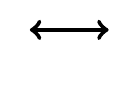
\begin{tikzpicture}
 \draw[ultra thick][<->] (-0.5,0)--(0.5,0);
 \draw[white] (-0.5,-0.5)--(0.5,-0.5);
\end{tikzpicture}
 \end{minipage}
 \begin{minipage}[b]{0.35\linewidth}
  \centering
  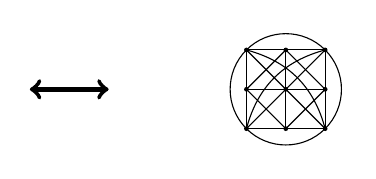
\begin{tikzpicture}
 \draw[ultra thick][<->] (-3.25,0)--(-2.25,0);
 \draw (-0.5,-0.5)--(-0.5,0.5);
 \draw (0,-0.5)--(0,0.5);
 \draw (0.5,-0.5)--(0.5,0.5);
 \draw (-0.5,-0.5)--(0.5,-0.5);
 \draw (-0.5,0)--(0.5,0);
 \draw (-0.5,0.5)--(0.5,0.5);
 \draw (-0.5,-0.5)--(0.5,0.5);
 \draw (-0.5,0.5)--(0.5,-0.5);
 \draw (-0.5,0)--(0,0.5);
 \draw (-0.5,0)--(0,-0.5);
 \draw (0.5,0)--(0,0.5);
 \draw (0.5,0)--(0,-0.5);
 \draw (-0.5,0.5) to [out=45,in=135] (0.5,0.5);
 \draw (0.5,0.5) to [out=315,in=45] (0.5,-0.5);
 \draw (0.5,-0.5) to [out=225,in=315] (-0.5,-0.5);
 \draw (-0.5,-0.5) to [out=135,in=225] (-0.5,0.5);
 \draw (-0.5,-0.5) to [out=75,in=195] (0.5,0.5);
 \draw (-0.5,0.5) to [out=345,in=105] (0.5,-0.5);
 \foreach \x in {-0.5,0,0.5}
  \foreach \y in {-0.5,0,0.5}
   \fill (\x,\y) circle (0.03);
\end{tikzpicture}
 \end{minipage}
 \caption{チェス盤とクイーングラフの対応関係}
\end{figure}

\begin{table}[hbtp]
   \centering
   \caption{$n$と$\gamma(Q_n)$の上下限}
   \begin{tabular}{c|c||c|c||c|c||c|c||c|c} \hline
    $n$ & $\gamma(Q_{n})$ & $n$ & $\gamma(Q_{n})$ &$n$ & $\gamma(Q_{n})$ &$n$ & $\gamma(Q_{n})$ &$n$ & $\gamma(Q_{n})$ \\ \hline \hline
    1 &1 &6 &3 &11 &5 &16 &9 &21 &11\\ \hline
    2 &1 &7 &4 &12 &6 &17 &9 &22 &12\\ \hline
    3 &1 &8 &5 &13 &7 &18 &9 &23 &12\\ \hline
    4 &2 &9 &5 &14 &8 &19 &10 &24 &13\\ \hline
    5 &3 &10 &5 &15 &9 &20 &11 &25 &13\\ \hline
   \end{tabular}
   \label{tb:queen_n}
  \end{table}


\begin{figure}[htb]
  \centering
  \begin{tikzpicture}
 \draw[gray] (-1.25,-1.25)--(-1.25,1.25);
 \draw[gray] (-0.75,-1.25)--(-0.75,1.25);
 \draw[gray] (-0.25,-1.25)--(-0.25,1.25); 
 \draw[gray] (0.25,-1.25)--(0.25,1.25); 
 \draw[gray] (0.75,-1.25)--(0.75,1.25); 
 \draw[gray] (1.25,-1.25)--(1.25,1.25); 
 \draw[gray] (-1.25,-1.25)--(1.25,-1.25); 
 \draw[gray] (-1.25,-0.75)--(1.25,-0.75); 
 \draw[gray] (-1.25,-0.25)--(1.25,-0.25); 
 \draw[gray] (-1.25,0.25)--(1.25,0.25); 
 \draw[gray] (-1.25,0.75)--(1.25,0.75); 
 \draw[gray] (-1.25,1.25)--(1.25,1.25);
 \foreach \x in {-1,-0.5,0,0.5,1}
  \foreach \y in {-1,-0.5,0,0.5,1} 
  \fill (\x,\y) circle (0.03);
 \draw[magenta] (-1.25,1)--(1.25,1);
 \draw[magenta] (-1,1.25)--(-1,-1.25);
 \draw[magenta] (-1.25,1.25)--(1.25,-1.25);
 \draw[magenta] (-1.25,0.75)--(-0.75,1.25);
 \draw[blue] (-1.25,-1)--(1.25,-1);
 \draw[blue] (-0.5,-1.25)--(-0.5,1.25);
 \draw[blue] (-0.25,-1.25)--(-1.25,-0.25);
 \draw[blue] (-0.74,-1.25)--(1.25,0.74);
 \draw[yellow] (1,1.25)--(1,-1.25);
 \draw[yellow] (-1.25,0.5)--(1.25,0.5);
 \draw[yellow] (0.25,1.25)--(1.25,0.25);
 \draw[yellow] (-0.76,-1.25)--(1.25,0.76);
 \fill[magenta] (-1,1) circle (0.03);
 \fill[yellow] (1,0.5) circle (0.03);
 \fill[blue] (-0.5,-1) circle (0.03);
  \matrix[matrix of nodes,nodes={inner sep=0pt,text width=0.5cm,
align=center,minimum height=0.43cm}]{
 \textcolor{magenta}{\symqueen} & \quad & \quad & \quad & \quad \\
 \quad & \quad & \quad & \quad & \textcolor{yellow}{\symqueen} \\
 \quad & \quad & \quad & \quad & \quad \\
 \quad & \quad & \quad & \quad & \quad \\
 \quad & \textcolor{blue}{\symqueen} & \quad & \quad & \quad \\};
\end{tikzpicture}
 

  \caption{$Q_5$の最小支配集合の例}
  \label{ex:queengraph5}
\end{figure}

%%% Local Variables:
%%% mode: latex
%%% TeX-master: "paper"
%%% End:
